% Final report, Multimedia Systems course -- IEEE conference format (IEEEtran).
% Build:  tectonic main.tex      (or upload paper/ to Overleaf, compiler pdfLaTeX)
%
% \todo{...} is a writing note and prints in red; \tbd marks a number that waits
% for an experiment. Search for both before submitting: none may remain.
\documentclass[conference]{IEEEtran}
% Vietnamese text is typed directly in UTF-8 inside \vi{...}.
% pdfLaTeX (Overleaf default) uses the T5 font encoding; XeLaTeX/LuaLaTeX and Tectonic use a Unicode Times clone.
\usepackage{iftex}
\ifPDFTeX
  \usepackage[utf8]{inputenc}
  \usepackage[T5,T1]{fontenc}
  \newcommand{\vi}[1]{{\fontencoding{T5}\selectfont #1}}
\else
  \usepackage{fontspec}
  \setmainfont{texgyretermes}[Extension=.otf, UprightFont=*-regular, BoldFont=*-bold,
    ItalicFont=*-italic, BoldItalicFont=*-bolditalic, Ligatures=TeX]
  \newcommand{\vi}[1]{#1}
\fi
\usepackage{cite}
\usepackage{amsmath,amssymb}
\usepackage{graphicx}
\usepackage{booktabs}
\usepackage{xcolor}
\usepackage{url}

\newcommand{\todo}[1]{\textcolor{red}{[#1]}}
\newcommand{\tbd}{\textcolor{red}{--}}


% Numbers measured locally on the 192 single-image test infographics
% (scripts/locator_stats.py). Re-run the script and update here if anything changes.
\newcommand{\MedianWidth}{1{,}270}
\newcommand{\MedianMP}{3.3}
\newcommand{\MedianDown}{1.8}
\newcommand{\MedianZoom}{1.8}

\begin{document}

\title{Format, Not Pixels: A Training-Free Diagnosis of a Small Vision-Language Model on Vietnamese Infographic Question Answering}

\author{
\IEEEauthorblockN{Ngo Truong Minh Dat}
\IEEEauthorblockA{\textit{Faculty of Information Technology} \\
\textit{University of Science, VNU-HCM}\\
Ho Chi Minh City, Vietnam \\
25C1500308@student.hcmus.edu.vn}
\and
\IEEEauthorblockN{Nguyen Dinh Loc}
\IEEEauthorblockA{\textit{Faculty of Information Technology} \\
\textit{University of Science, VNU-HCM}\\
Ho Chi Minh City, Vietnam \\
25C1105079@student.hcmus.edu.vn}
}

\maketitle

\begin{abstract}
Infographics pack text, charts, maps and icons into dense layouts, and answering questions about them requires reading small text as much as reasoning. On ViInfographicVQA, the first Vietnamese benchmark for this task, fine-tuning a 7B vision-language model was reported to improve the score by about one point only, which suggests that supervision is not the bottleneck. We study a 3B model, Qwen2.5-VL-3B, without any training and test two other suspects: the resolution at which the model sees the image, and the format in which it is expected to answer. For resolution, we add OCR text to the prompt, and we use OCR as a \emph{locator} that selects regions of the full-resolution image to show to the model alongside the whole image. Neither changes the score: the baseline reaches 62.37 ANLS, OCR text 62.06 and located crops 62.12, although the crops contain the reference answer for 66\% of the questions whose answer OCR can read, and cost 1.8 times the visual tokens. For format, five rules derived from the conventions of the training answers raise the score to 64.75 (+2.38, 95\% interval $[+0.7, +4.0]$) at no extra cost, which closes almost half of the gap to the reported 7B zero-shot result of 67.42. We also show that the benchmark's released scorer is more lenient than the ANLS metric it is described as, by about eight points on our predictions, and report both. On this benchmark, how a small model expresses its answer and how that answer is scored matter more than how many pixels the model sees.
\end{abstract}

\begin{IEEEkeywords}
visual question answering, infographics, Vietnamese, vision-language models, optical character recognition, visual cropping, evaluation
\end{IEEEkeywords}

%=====================================================================
\section{Introduction}
Infographics are a common way to communicate statistics, schedules, forecasts and procedures to the public. A single image combines running text, charts, maps, tables and pictograms in a free layout, so answering a question about it requires locating the relevant element, reading it, and often counting or computing. Infographic question answering has therefore become a demanding test for vision-language models (VLMs)~\cite{infographicvqa}. Resources for it are overwhelmingly English; ViInfographicVQA~\cite{viinfographicvqa} is the first benchmark for Vietnamese, with 20{,}409 question--answer pairs over 6{,}747 infographics published by the Vietnam News Agency.

One result in the benchmark paper motivates this work. The authors fine-tune Qwen2.5-VL-7B on the 12{,}521 single-image training questions and the single-image score moves from 67.42 to 67.80; training on the single- and multi-image data together gives 68.53~\cite{viinfographicvqa}. Thousands of in-domain examples buy about one point. If more supervision barely helps, the errors are unlikely to come from a lack of task knowledge, and the question becomes what does limit these models.

We examine two candidates. The first is perception. The infographics are dense and often large: the median test image is \MedianWidth{}\,px wide and has \MedianMP{} megapixels, and the largest has 28.9. Under the benchmark's evaluation protocol the model receives at most 1{,}280 visual tokens, about one megapixel, so 88\% of the test images are downscaled before the model sees them, by a median factor of \MedianDown{} and up to 5.4 in each dimension. If small labels and numbers, which are exactly what many questions ask for, become unreadable, no amount of fine-tuning on the same downscaled inputs can recover them. The second is answer format. The benchmark scores string similarity against a single reference, and many predictions that are correct in substance receive no credit: ``\vi{10 ngày}'' (10 days) for the reference ``10'', or a paraphrase where the reference copies the text of the image. The prompt used in the benchmark paper also asks for ``a single term'', although a quarter of the questions expect a list.

We test both without training, on a 3B model that fits a free 16\,GB GPU. For format, we replace the prompt with explicit rules derived from the conventions of the training answers. For perception, we compare two uses of optical character recognition (OCR). The conventional one appends the recognised text to the prompt. Vietnamese OCR, however, frequently gets diacritics and digits wrong, and that noise is handed directly to the model. The second uses OCR as a \emph{locator}: question words are matched against the recognised text boxes, with diacritics ignored and small spelling errors tolerated, and the best-matching regions are cropped from the full-resolution image and given to the model together with the whole image. OCR decides where to look; the model does the reading.

The outcome separates the two candidates clearly. The format rules raise the score of the 3B model from 62.37 to 64.75 ANLS, a larger change than the one reported for fine-tuning the 7B model, and they do so on exactly the question types where the baseline's answers were malformed. Neither use of OCR changes the score, even though the locator places the reference answer inside its crops for two thirds of the questions whose answer OCR can read. At the benchmark's pixel budget, the small model's errors are mostly not errors of resolution.

Our contributions are:
\begin{itemize}
\item an analysis of the errors of a small VLM on ViInfographicVQA that separates arithmetic, misread details, incomplete lists and format mismatches (Section~\ref{sec:errors});
\item answer-format rules derived from the training split, which improve the score by 2.38 points without training or extra computation (Section~\ref{sec:format});
\item a negative result on resolution: OCR text in the prompt and OCR-as-locator zoom, a cropping method that needs no extra model call and no access to model internals, both leave the score unchanged (Sections~\ref{sec:ocrtext} and~\ref{sec:zoom});
\item an audit of the benchmark's scorer, which we show to be more lenient than the ANLS definition given in the benchmark paper (Section~\ref{sec:metric}).
\end{itemize}

%=====================================================================
\section{Related Work}

\subsection{Document and Infographic VQA}
Text-centric visual question answering began with scene text. TextVQA~\cite{textvqa} and ST-VQA~\cite{stvqa} showed that general VQA models could not read, and ST-VQA introduced the Average Normalized Levenshtein Similarity (ANLS) to tolerate small recognition errors. DocVQA~\cite{docvqa} moved the task to scanned documents, ChartQA~\cite{chartqa} to real-world charts with human-written questions, and InfographicVQA~\cite{infographicvqa} to infographics, where answers frequently require combining text, layout and elementary arithmetic. All of these are English.

\subsection{Vietnamese VQA}
Vietnamese resources have followed a similar path at a smaller scale: ViVQA~\cite{vivqa} for natural images, OpenViVQA~\cite{openvivqa} for open-ended answers, ViTextVQA~\cite{vitextvqa} for scene text, and the document and OCR collections released with Vintern-1B~\cite{vintern}. ChartTableViVQA~\cite{charttablevivqa} covers charts and tables. ViInfographicVQA~\cite{viinfographicvqa} is the first benchmark on Vietnamese infographics and adds a multi-image task. Its authors evaluate seven open VLMs of 5--9B parameters zero-shot and fine-tune one of them. They do not study smaller models, prompting, or the effect of input resolution, which are the subject of this paper.

\subsection{High-Resolution Perception by Visual Cropping}
A VLM encodes an image with a bounded number of visual tokens, so details in large images are lost. One family of remedies changes the model, by tiling the input or training at higher resolution. Another leaves the model unchanged and adds a second, zoomed view of the relevant region at inference time. ViCrop~\cite{vicrop} observes that models often attend to the right region even when they answer wrongly, and derives the crop from the model's own attention and gradient maps. HAVC~\cite{havc} refines the choice of attention heads used for this purpose. TextCoT~\cite{textcot} instead asks the model to output the bounding box of the answer region in a first pass and answers from the crop in a second. These methods need either access to model internals or additional forward passes. Our locator is external and lexical: it reuses a single OCR pass per image, costs no model call, and is designed around the specific weakness of OCR in a language with diacritics.

\subsection{OCR-Augmented Models}
Feeding recognised text to the model is the classical recipe in text-centric VQA, from pointer networks over OCR tokens~\cite{m4c} to prompts that include the OCR transcript. Its quality is bounded by the OCR engine. We keep this recipe as a comparison point (Section~\ref{sec:ocrtext}) and contrast it with using the same OCR output for position only.

%=====================================================================
\section{Benchmark and Baseline}

\subsection{Dataset}
ViInfographicVQA~\cite{viinfographicvqa} collects infographics from the Vietnam News Agency's infographics portal across nine topics, including economy, health, society, weather forecasts and sport. Questions and answers were generated with a VLM-assisted pipeline and then verified by annotators. The single-image task pairs each question with one infographic; the multi-image task requires evidence from two to four related infographics. Table~\ref{tab:data} gives the sizes of the released splits. We use the single-image task: 1{,}374 test questions on 192 images, about seven questions per image.

Each single-image question carries two labels that we use throughout. The \emph{answer source} says how the answer relates to the inputs: \emph{image-span} (copied from the image), \emph{question-span} (one of the options listed in the question), \emph{multi-span} (several items) and \emph{non-extractive} (obtained by counting or computing). The four types are balanced in the test set, with 359, 332, 341 and 342 questions respectively. The \emph{element} label names the part of the infographic that holds the evidence: text, diagram or graph, map, table, sequence, or visual/layout. Fig.~\ref{fig:dataset} shows the distribution of elements and topics in the test set.

\begin{figure}[t]
\centering
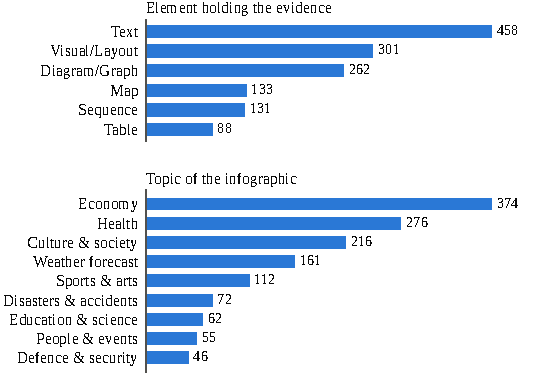
\includegraphics[width=\columnwidth]{figs/fig_dataset.pdf}
\caption{The 1{,}374 single-image test questions by the element that holds the evidence and by the topic of the infographic.}
\label{fig:dataset}
\end{figure}

\begin{table}[t]
\caption{ViInfographicVQA splits (counts from the released annotation files).}
\label{tab:data}
\centering
\begin{tabular}{lrr}
\toprule
Split & Questions & Images \\
\midrule
Single-image, train & 12{,}521 & 1{,}788 \\
Single-image, test  & 1{,}374  & 192 \\
Multi-image, train  & 5{,}878  & 4{,}823 \\
Multi-image, test   & 636      & 509 \\
\bottomrule
\end{tabular}
\end{table}

\subsection{Baseline Model and Protocol}
\label{sec:baseline}
Our model is Qwen2.5-VL-3B~\cite{qwen25vl}, the smallest member of the family whose 7B variant is the strongest fine-tunable baseline in the benchmark paper. Qwen2.5-VL encodes an image at its native aspect ratio, one visual token per $28\times28$ pixels, within a configurable pixel budget; larger images are downscaled to fit.

The baseline reproduces the benchmark's protocol as released in its code: the system prompt ``Answer the following question based solely on the image content concisely with a single term'', a user turn holding the image and the question, an image budget between 256 and 1{,}280 visual tokens ($1{,}280 \times 28^2 \approx 1.0$ megapixel), and at most 100 generated tokens. We differ in two respects: the model has 3B instead of 7B parameters, and we decode greedily so that runs are reproducible.

Fig.~\ref{fig:resolution} relates this budget to the size of the test images. Only 12\% of them fit within it; the rest are downscaled, the median image by a factor of \MedianDown{} in each dimension.

\begin{figure}[t]
\centering
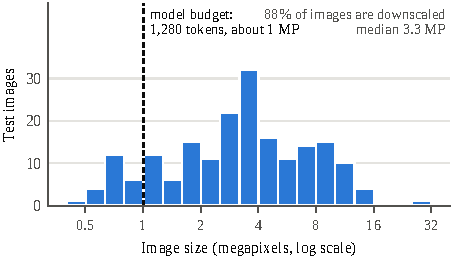
\includegraphics[width=\columnwidth]{figs/fig_resolution.pdf}
\caption{Size of the 192 single-image test infographics compared with the pixel budget of the evaluation protocol. Images to the right of the dashed line are downscaled before the model sees them.}
\label{fig:resolution}
\end{figure}

\subsection{Metric}
\label{sec:metric}
The benchmark reports ANLS~\cite{stvqa}. For a prediction $p$ and reference $g$,
\begin{equation}
s(p, g) =
\begin{cases}
1 - \mathrm{NL}(p, g) & \text{if } \mathrm{NL}(p, g) < 0.5,\\
0 & \text{otherwise,}
\end{cases}
\label{eq:anls}
\end{equation}
where $\mathrm{NL}$ is the Levenshtein distance divided by the length of the longer string, and the score is the mean of $s$ over questions.

The released scorer does not implement~\eqref{eq:anls}. It computes the similarity ratio $1 - d_{\mathrm{indel}}(p, g) / (|p| + |g|)$, where $d_{\mathrm{indel}}$ counts insertions and deletions only, and keeps it when it is at least 0.5. The two agree on identical strings but the ratio is more generous when the strings differ in length. For the prediction ``\vi{hà nội}'' against the reference ``\vi{hà nội và đà nẵng}'', equation~\eqref{eq:anls} gives 0, while the released scorer gives 0.52. On 200{,}000 random string pairs the released similarity was never lower than $1 - \mathrm{NL}$ and was strictly higher for 93\% of them.

We therefore report three numbers for every run: the released scorer, which we verified to reproduce the official implementation exactly on all test questions and which makes our results comparable with the published ones (``ANLS''); the textbook definition~\eqref{eq:anls} (``ANLS-std''); and exact match after the same normalisation (``EM'').

%=====================================================================
\section{Method}

\subsection{Error Analysis of the Baseline}
\label{sec:errors}
The baseline of Section~\ref{sec:baseline} scores zero on 412 of the 1{,}374 test questions. We drew 100 of them at random and labelled each by comparing the question, the reference and the prediction; the labels are released with the code. Five kinds of error appear.

\emph{Arithmetic and counting (28\%).} The question asks for a sum, a difference or a count of items or icons, and the number is wrong.

\emph{Misread detail (27\%).} The answer has the right form but the wrong content: a figure read from the wrong row of a table, one region of a weather map confused with its neighbour, or the wrong option in a question that offers two.

\emph{Wrong or incomplete list (26\%).} The question asks for several items and the model returns one of them, a different set, or, in four cases, the sum of the values it was asked to list.

\emph{Format mismatch (17\%).} The answer is right but not in the reference's form. The model writes ``\vi{10 ngày}'' where the reference is ``10'', ``2018'' where it is ``\vi{(sinh năm 2018)}'', or a two-word answer where the reference repeats the full sentence printed on the image.

\emph{Other (2\%).} One reference is itself mistyped and one prediction is off-topic text.

The format and list errors, 43\% of the sample, concern how the answer is expressed and are addressed in Section~\ref{sec:format}; the misread details concern what the model can see and are addressed in Sections~\ref{sec:ocrtext} and~\ref{sec:zoom}. None of our techniques targets the arithmetic and counting errors directly. The sample covers only answers that score zero; among the 377 answers with partial credit, differences of form are likely to be more frequent.

\subsection{Answer-Format Prompting}
\label{sec:format}
The reference answers follow consistent conventions, which we measured on the training split only. Of the 3{,}058 non-extractive training answers, 99.0\% are a bare number without unit. Of the 3{,}087 multi-span answers, 98.5\% are comma-separated lists, with a median length of eight words. Image-span answers copy the wording of the image, units included (``23,1\%'', ``998 mb''), and question-span answers copy one of the options given in the question.

We replace the instruction ``with a single term'' by five rules that state these conventions: (i) for a count or a calculation, answer with the number only; (ii) copy a value shown in the image exactly, including its unit; (iii) copy text shown in the image exactly, without paraphrasing or translating; (iv) when the question offers options, answer with the chosen option as written in the question; (v) when several items are asked for, list all of them, separated by commas. The model is not told the answer type of a question; it must decide which rule applies.

\subsection{OCR Text Augmentation}
\label{sec:ocrtext}
We run EasyOCR~\cite{easyocr} with its Vietnamese model on each image, resized so that its longer side is at most 2{,}560 pixels, which is well above the resolution the VLM receives. Detections with confidence below 0.3 are discarded. The remaining boxes are grouped into lines by vertical position and read left to right, and the resulting transcript, truncated to 3{,}000 characters, is inserted before the question with a note that it may contain errors and that the image takes precedence.

The transcript is imperfect in three ways. Diacritics are often wrong (``\vi{Phân trăm}'' for ``\vi{Phần trăm}''), digits and symbols are confused (``8,99'' for ``8,9\%''), and reading boxes line by line destroys column structure, so a label and its value may end up far apart.

\subsection{OCR as a Locator}
\label{sec:zoom}
The errors above affect what the OCR text \emph{says} much more than \emph{where} it is. A box read as ``\vi{BỔ ĐÀO NHA}'' instead of ``\vi{BỒ ĐÀO NHA}'' is a poor source for the answer but an excellent pointer to the panel about Portugal. This suggests using the OCR output only to choose regions of the original image, and letting the model read those regions itself at higher magnification. Fig.~\ref{fig:example} shows the result for one question.

\begin{figure}[t]
\centering
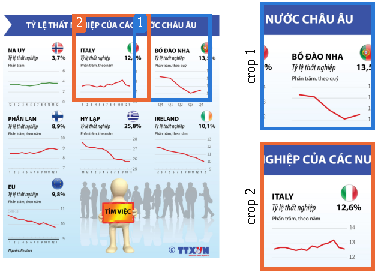
\includegraphics[width=\columnwidth]{figs/fig_example.pdf}
\caption{OCR as a locator for the question ``Is Portugal's unemployment rate given per year or per quarter?'' (asked in Vietnamese). Left: the infographic with the two selected windows. Right: the crops given to the model in addition to the whole image. Crop~1 contains the answer (``\vi{Phần trăm, theo quý}''); crop~2 was selected because it repeats the words ``unemployment rate''.}
\label{fig:example}
\end{figure}

\subsubsection{Matching}
Question and box texts are lowercased, stripped of diacritics and split into words and numbers. A question word $t$ matches a box $b$ with strength $m(t, b) \in [0, 1]$: 1 if the word occurs in the box, otherwise the highest string similarity to a word of the box if that similarity is at least 0.8, and 0 otherwise. Numbers and words shorter than four characters must match exactly.

\subsubsection{Box relevance}
Not all matches are equally informative. Each question word receives the weight
\begin{equation}
w(t) = \frac{\mathrm{idf}(t)}{\mathrm{idf}_{\max}} \cdot \log\!\Big(1 + \frac{|B|}{n_t}\Big),
\end{equation}
where $\mathrm{idf}(t)$ is the inverse document frequency of $t$ over the benchmark's questions, which removes function words and stock phrases such as ``\vi{bao nhiêu}'' (how many); $B$ is the set of boxes of the image; and $n_t$ is the number of boxes that match $t$, so that a word printed all over the image counts less than one that occurs in a single place. The relevance of a box is
\begin{equation}
r(b) = \Big(\sum_{t \in q} w(t)\, m(t, b)\Big)\,\big(0.5 + c(b)\big),
\end{equation}
where $c(b)$ is the fraction of the box's words that occur in the question. The second factor favours a short label that the question names in full over a long sentence that happens to share a few words with it.

\subsubsection{Window selection}
Every box with $r(b) > 0$ proposes a window centred on it, spanning a fraction $\rho$ of the image width and height and shifted to stay inside the image. A window is scored by the total relevance of the boxes whose centres it contains. Windows are selected greedily in decreasing score, skipping any window whose intersection-over-union with an already selected one exceeds 0.3, until $K$ windows are chosen. We use $K = 2$ and $\rho = 0.35$, so the crops together cover at most a quarter of the image. If no box matches the question, no crop is produced and the model answers from the whole image as in the baseline.

\subsubsection{Model input}
The user turn contains the whole image under the baseline budget of 1{,}280 tokens, followed by each crop, taken from the original full-resolution image, under a budget of 768 tokens, a sentence stating that the later images are enlarged regions of the first, and the question. For the median test image, a crop is shown at \MedianZoom{} times the linear magnification of the whole-image view. The global view is kept because many questions depend on overall layout, and because the locator can be wrong.

\subsection{Controls}
\label{sec:controls}
A gain from adding crops could come from looking at the right place or simply from giving the model more pixels. Two controls would separate these: \emph{random crops}, with the same number and size of windows at positions drawn uniformly at random, and a \emph{grid} that splits the image into $2 \times 2$ tiles and adds all four. We use random crops to evaluate the locator itself, without the VLM (Section~\ref{sec:locator}). We did not run either control end to end: a zoom run takes about seven hours on a free GPU, grid tiling costs 3.1 times the visual tokens of the baseline (Section~\ref{sec:cost}), and, as Section~\ref{sec:results} shows, the located crops produced no gain that a control would need to explain.

%=====================================================================
\section{Experimental Setup}
All runs use the public Qwen2.5-VL-3B-Instruct checkpoint in bfloat16 precision on a single 16\,GB GPU of the free tiers of Google Colab and Kaggle. No model is trained or fine-tuned. Every configuration answers the same 1{,}374 single-image test questions with greedy decoding and at most 100 new tokens, and differs from the baseline of Section~\ref{sec:baseline} only in the component under study. OCR is run once per image and cached, and the OCR-text and locator configurations use the same OCR engine and settings. Table~\ref{tab:setup} lists the settings. Code and notebooks are available at \url{https://github.com/ngotruongminhdat/MultiMedia}.

\begin{table}[t]
\caption{Settings shared by all runs.}
\label{tab:setup}
\centering
\begin{tabular}{ll}
\toprule
Setting & Value \\
\midrule
Model & Qwen2.5-VL-3B-Instruct \\
Whole-image budget & 256--1{,}280 tokens \\
Crop budget & up to 768 tokens each \\
Decoding & greedy, 100 new tokens \\
OCR engine & EasyOCR, Vietnamese + English \\
OCR input size & longer side 2{,}560\,px \\
OCR confidence threshold & 0.3 \\
OCR text limit (text mode) & 3{,}000 characters \\
Crops $K$, size $\rho$ & 2, 0.35 \\
Fuzzy match threshold & 0.8 \\
Window overlap limit (IoU) & 0.3 \\
\bottomrule
\end{tabular}
\end{table}

%=====================================================================
\section{Results}
\label{sec:results}

\subsection{Main Results}
Table~\ref{tab:main} gives the results. The 3B baseline reaches 62.37 ANLS under the released scorer, 5.05 points below the zero-shot 7B model of~\cite{viinfographicvqa} with the same prompt and pixel budget. Under the textbook definition the same predictions score 54.44, so the choice of scorer alone moves the result by 7.93 points.

\emph{OCR text does not help.} Adding the recognised text to the prompt leaves the score where it was: 62.06 ANLS against 62.37. A paired bootstrap over the 1{,}374 questions (10{,}000 resamples) gives a 95\% interval of $[-1.7, +1.1]$ points for the difference, so it is not distinguishable from zero. The text is not ignored. It changes the prediction for 487 questions, but the score rises for 133 of them and falls for 167, and the two effects cancel. By element, questions on maps and tables gain about two points (58.43 to 60.65 and 66.27 to 68.21), where the evidence is a short printed label or cell, while questions on charts and on visual layout lose more than one point each. Noisy Vietnamese OCR, flattened into a single string without its layout, is therefore not a reliable second source for the answer itself.

\emph{Format rules help.} Replacing the single-term instruction with the five answer-format rules raises ANLS from 62.37 to 64.75 (+2.38; 95\% paired-bootstrap interval $[+0.7, +4.0]$), textbook ANLS by 2.79 and exact match by 3.71 points, at no extra cost in visual tokens. The rules change 483 predictions; the score rises for 195 questions and falls for 119. The gain is concentrated where the error analysis of Section~\ref{sec:errors} placed it: multi-span questions improve from 52.71 to 60.37 ANLS and from 18.48\% to 28.15\% exact match, and image-span questions from 69.18 to 72.22. Non-extractive questions barely move (54.88 to 55.37), which is consistent with their errors being errors of arithmetic and counting, not of form. Question-span questions lose 1.81 points. With the rules, the gap to the 7B zero-shot model narrows from 5.05 to 2.67 points.

\emph{Zooming does not help.} Adding the two OCR-located crops gives 62.12 ANLS against 62.37 for the baseline, a difference of the same size as the one for OCR text and well inside its interval. Textbook ANLS and exact match move in the opposite direction, by $+0.38$ and $+1.02$ points, so the sign of the effect depends on the metric. The crops are not useless everywhere: image-span questions gain 1.73 points and questions on tables 6.63, the two places where reading a small printed value is the whole task, but multi-span questions lose 2.15 and question-span questions 1.34 (Table~\ref{tab:breakdown}). The model thus pays 1.8 times the visual tokens (Section~\ref{sec:cost}) for no net gain. We did not have the per-question predictions of this run available for a bootstrap interval.

\begin{table}[t]
\caption{Single-image test results (1{,}374 questions). ANLS: released scorer; ANLS-std: textbook definition; EM: exact match. The first three rows are quoted from~\cite{viinfographicvqa}.}
\label{tab:main}
\centering
\begin{tabular}{lrrr}
\toprule
Method & ANLS & ANLS-std & EM \\
\midrule
\multicolumn{4}{l}{\textit{Reported in~\cite{viinfographicvqa}}} \\
Qwen2.5-VL-7B, zero-shot   & 67.42 & -- & -- \\
Qwen2.5-VL-7B, fine-tuned  & 67.80 & -- & -- \\
Ovis2.5-9B                 & 71.02 & -- & -- \\
\midrule
\multicolumn{4}{l}{\textit{Ours, Qwen2.5-VL-3B, no training}} \\
Baseline (paper prompt)          & 62.37 & 54.44 & 42.58 \\
+ format rules                   & 64.75 & 57.23 & 46.29 \\
+ OCR text                       & 62.06 & 53.63 & 41.99 \\
+ zoom, OCR-located crops        & 62.12 & 54.82 & 43.60 \\
\bottomrule
\end{tabular}
\end{table}

\subsection{Breakdown by Answer Type and Element}
Table~\ref{tab:breakdown} splits the score by answer type and by element. The format rules improve every element and three of the four answer types; their largest gains are on multi-span answers ($+7.66$) and on tables ($+5.86$). The two OCR-based techniques have no consistent direction: each helps some groups and hurts others by one to two points, which is what a change without systematic effect looks like on groups of 88 to 458 questions. Non-extractive questions stay between 54.4 and 55.5 under every technique.

\begin{table}[t]
\caption{ANLS (released scorer) by answer type and by element. Base: baseline; Format: format rules; Text: OCR text in the prompt; Zoom: OCR-located crops.}
\label{tab:breakdown}
\centering
\begin{tabular}{lrrrrr}
\toprule
 & $n$ & Base & Format & Text & Zoom \\
\midrule
\multicolumn{6}{l}{\textit{Answer type}} \\
Image-span     & 359 & 69.18 & \textbf{72.22} & 68.53 & 70.91 \\
Question-span  & 332 & 72.63 & 70.82 & \textbf{74.06} & 71.29 \\
Multi-span     & 341 & 52.71 & \textbf{60.37} & 51.26 & 50.56 \\
Non-extractive & 342 & 54.88 & 55.37 & 54.38 & \textbf{55.52} \\
\midrule
\multicolumn{6}{l}{\textit{Element}} \\
Text           & 458 & 64.14 & \textbf{66.15} & 63.68 & 63.09 \\
Visual/Layout  & 301 & 55.25 & \textbf{57.82} & 54.00 & 54.67 \\
Diagram/Graph  & 262 & 66.29 & \textbf{67.90} & 64.94 & 64.89 \\
Map            & 133 & 58.43 & 59.74 & \textbf{60.65} & 59.62 \\
Sequence       & 131 & 65.72 & \textbf{69.31} & 66.17 & 65.34 \\
Table          &  88 & 66.27 & 72.13 & 68.21 & \textbf{72.90} \\
\midrule
All            & 1{,}374 & 62.37 & \textbf{64.75} & 62.06 & 62.12 \\
\bottomrule
\end{tabular}
\end{table}

\subsection{Locator Quality}
\label{sec:locator}
Before measuring answers, we ask how often the locator points at the right place. This can be estimated without running the VLM. We call a question \emph{OCR-readable} if at least 80\% of the words of its reference answer occur, up to diacritics and small errors, in the OCR boxes of the image, and say that the answer is \emph{inside the crops} if the same holds for the boxes within the selected windows. The reference answers are used here only to evaluate the locator, never to choose the windows.

Of the 1{,}374 test questions, 1{,}010 (73.5\%) are OCR-readable; the share is 88\% for image-span and 93\% for multi-span answers, and 39\% for non-extractive ones, whose answers are computed and usually not printed on the image. Fig.~\ref{fig:locator} shows the result for these questions. The two located crops contain the answer for 66.0\% of them, against 27.9\% for two random crops of the same size, which cover the same quarter of the image. The locator is strongest on question-span questions (87.7\%), where the options named in the question are printed on the image and act as anchors, and weakest on multi-span questions (44.5\%), whose answers are spread over more of the image than two windows can cover. It selects 1.95 windows per question on average and finds no match, falling back to the whole image alone, for 0.9\% of the questions.

\begin{figure}[t]
\centering
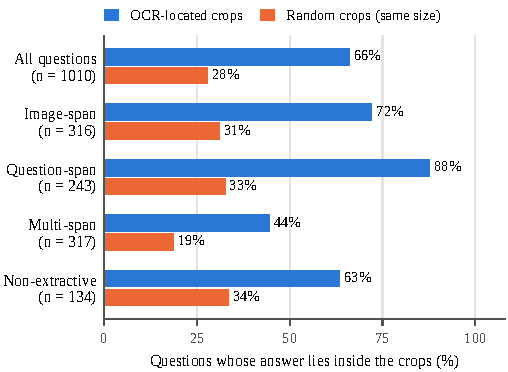
\includegraphics[width=\columnwidth]{figs/fig_locator.pdf}
\caption{Share of OCR-readable test questions whose reference answer lies inside the crops, for OCR-located crops and for random crops of the same number and size, by answer type.}
\label{fig:locator}
\end{figure}

Set against Table~\ref{tab:breakdown}, these figures show that finding the right region is not what limits the model. The change in score does not follow the locator's accuracy: the locator is most accurate on question-span questions, yet these lose 1.34 points when the crops are added, while multi-span questions, where it is least accurate, lose 2.15. Only image-span questions, where the answer is a printed string and the crops contain it for 72\% of the readable questions, improve. A magnified view of the right region helps when the difficulty is reading a string, and that is a minority of the baseline's errors (Section~\ref{sec:errors}).

\subsection{Cost}
\label{sec:cost}
Zooming is not free: every crop adds visual tokens. Table~\ref{tab:cost} gives the number of visual tokens per question, counted with the model's own preprocessor over all 1{,}374 test questions. Two located crops raise the mean from 1{,}210 to 2{,}232 tokens, a factor of 1.8; the crops use fewer than their 768-token budget because, for most images, a window of this size already fits at native resolution. Grid tiling would cost 3{,}766 tokens, 3.1 times the baseline, and was not run for that reason. Random crops have the same size as located crops and therefore the same cost. OCR adds one pass of a lightweight detector and recogniser per image, shared by all questions on that image. In wall-clock terms, the run with located crops took 19 seconds per question on a free Kaggle GPU, about seven hours for the test set.

\begin{table}[t]
\caption{Visual tokens per question (1{,}374 test questions).}
\label{tab:cost}
\centering
\begin{tabular}{lrrr}
\toprule
Input & Mean & Median & Max \\
\midrule
Whole image (baseline) & 1{,}210 & 1{,}242 & 1{,}276 \\
+ 2 located crops      & 2{,}232 & 2{,}306 & 2{,}796 \\
+ grid $2\times2$      & 3{,}766 & 4{,}154 & 4{,}314 \\
\bottomrule
\end{tabular}
\end{table}

\subsection{Qualitative Examples}
Table~\ref{tab:examples} shows four questions on which the format rules change the outcome. In the first three, the baseline has read the image correctly and loses all credit to the form of its answer: a unit the reference omits, a list cut short after its first item, a unit the reference keeps. The fourth shows the cost of the rules and explains the loss on question-span questions in Table~\ref{tab:breakdown}. The question offers two options, but the model applies the rule about copying values from the image and answers with the number itself. Of the 22 short questions that the rules turn from fully right to fully wrong, six are of this kind, and nine are counts that came out differently.

\begin{table}[t]
\caption{Questions whose outcome the format rules change (questions translated; answers as produced). The first three are fixed by the rules, the last is broken.}
\label{tab:examples}
\centering
\small
\begin{tabular}{p{0.34\columnwidth}p{0.17\columnwidth}p{0.14\columnwidth}p{0.17\columnwidth}}
\toprule
Question & Reference & Baseline & Format \\
\midrule
How many days does exam registration last? & 10 & \vi{10 ngày} & 10 \\
\addlinespace
What does the map say about the stadium's location and construction dates? & \vi{bulacan, 2011 tháng 8, 2014 tháng 7} & Bulacan & \vi{Bulacan, 2011 tháng 8, 2014 tháng 7} \\
\addlinespace
Is the number of deaths reported for the day 0 or 1? & \vi{0 ca} & 0 & \vi{0 ca} \\
\addlinespace
Is the number of patients shown large or small? & \vi{lớn} & \vi{Lớn} & 104.793 \\
\bottomrule
\end{tabular}
\end{table}

%=====================================================================
\section{Discussion}
\textbf{What limits the small model.} The motivating observation was that fine-tuning buys little on this benchmark, and we asked whether resolution or answer format is the limit instead. For resolution the answer is negative. The whole-image view shrinks the median infographic by a factor of only \MedianDown{} in each dimension, and at that scale the model already reads most of the text it needs: a second view at \MedianZoom{} times the magnification, pointed at the right region for two thirds of the questions where this can be checked, does not change the score, and neither does handing the model the recognised text. Many of the misread details in the error analysis are values taken from the wrong row, region or series, which is an error of grounding and not of legibility. For format the answer is positive but partial. Stating the conventions of the reference answers recovers 2.38 points, more than the 0.38 points reported for fine-tuning the 7B model on the single-image training set, although the two numbers come from different model sizes and cannot be compared directly. What remains is dominated by counting and arithmetic, which no technique in this paper moves: non-extractive questions stay near 55 ANLS throughout.

\textbf{What the benchmark measures.} Two observations concern the evaluation itself. First, the released scorer gives the baseline 7.93 points more than the textbook ANLS it is described as, and the gap is similar for every configuration (7.3 to 8.4 points), so published numbers on this benchmark should not be compared with ANLS figures from other benchmarks. Second, small differences do not survive a change of metric. The format rules are the best configuration under all three metrics, but located crops rank below the baseline under the released scorer and above it under textbook ANLS and exact match. With 1{,}374 questions, the 95\% interval of a difference between two configurations is about three points wide; differences of a few tenths of a point, such as the one reported between zero-shot and fine-tuned models, are within that noise. Finally, 17\% of the zero-scoring answers we inspected were correct in substance, so a part of every score on this benchmark reflects agreement with the annotators' phrasing.

\textbf{Limitations.} We study one model, on the single-image task, with one OCR engine and one pixel budget. The negative result on zooming holds for a budget of 1{,}280 visual tokens and two crops of fixed size; under a tighter budget, or on the multi-image task where several infographics share the budget, resolution may matter more. Each configuration was run once, with greedy decoding. We ran neither the random-crop control nor the combination of format rules with located crops, and for the zoom run we could compute only aggregate scores, so its difference from the baseline comes without an interval. The locator is purely lexical: it cannot help with questions about pictures (``what does the icon on the phone show?'') or about position (``what is the first line of the text?''), and two crops cannot cover answers that are spread over the whole image. The box-relevance function was adjusted once after inspecting failures on 15 test images; the effect on locator quality was within one percentage point, but hyper-parameters should properly be tuned on the training split. Finally, the references of the benchmark were produced with VLM assistance and we did not quantify their noise, and the dataset is released without a licence, which restricts redistribution of the images.

%=====================================================================
\section{Conclusion}
We asked what limits a small vision-language model on Vietnamese infographic question answering when it is not trained on the task. With Qwen2.5-VL-3B on the single-image test set of ViInfographicVQA, stating the answer conventions of the benchmark in the prompt raises ANLS from 62.37 to 64.75 and closes almost half of the gap to a model more than twice its size. Giving the model more to read does not help: neither OCR text in the prompt (62.06) nor magnified crops selected by an OCR-based locator (62.12) changes the score, although the locator finds the region of the answer for two thirds of the questions it can be evaluated on. We also found that the benchmark's scorer is about eight points more generous than the metric it reports.

Several directions follow. Counting and arithmetic are the largest group of remaining errors and could be delegated to generated programs, as in program-of-thoughts learning~\cite{tinychart}. Multi-span answers still reach only 28\% exact match after the format rules, and a second pass that checks a list for completeness is a natural next step. The multi-image task, where reported scores are lowest and two to four infographics share the token budget, is the setting in which region selection is most likely to pay off. Finally, the benchmark itself would benefit from a scorer that matches its stated metric and from alternative references for answers that differ only in form.

\section*{Acknowledgment}
This work was carried out as the final project of the Multimedia Systems course at the University of Science, VNU-HCM. Experiments were run on the free tiers of Google Colab and Kaggle.

\bibliographystyle{IEEEtran}
\bibliography{refs}

\end{document}
